\chapter{Review of relevant literature} \label{cha:Literature-review}

\section{Introduction} \label{sec:Lit-Review-Introduction}

There are two major fields of literature relevant to this project: firstly, studies and technical reports delivered within engineering organisations relating to real spacecraft missions. Secondly, there has been a long history of theoretical study into optimising spacecraft trajectories, from early impulsive spacecraft research to more recent low-thrust scenarios.

% -------------------------------------------------------- Past missions --------------------------------------------------------
\section{Past missions} \label{sec:Past-missions}

% include review of \cite{Schoenmaekers2004} Post launch optimisation of SMART-1

While \textcite{LePage1991} shows that there have been numerous Earth-orbiting satellites using electric thrusters for attitude control or station keeping, only a small number of spacecraft have ever escaped the Earth's sphere of influence using electric propulsion as the primary thrust. These are listed in \autoref{tab:Past-low-thrust-missions}, along with key specifications of their respective propulsion systems. Thrust is the maximum force that the primary propulsion system can exert on the craft. Power consumption is the amount of electrical power used to operate at this maximum thrust. Specific impulse, $I_{sp}$, is the momentum added by the thrusters per unit weight-on-Earth of propellant, and consequently represents the fuel efficiency of the thrusters. Electric propulsion is characterised by relatively high $I_{sp}$.

\begin{table}[ht]
\caption{Past low-thrust missions to escape Earth's sphere of influence}
\label{tab:Past-low-thrust-missions}
\centering
\begin{minipage}{\textwidth}
\begin{tabular}{C{0.2\textwidth} C{0.25\textwidth} C{0.2\textwidth} C{0.1\textwidth} c}\toprule
  Spacecraft & Propulsion type & Total Power \linebreak Consumption \linebreak (W) & Total Thrust \linebreak (mN) & $I_{sp}$ (s)\\\midrule
  DS-1\footnote{\textcite{web_DS-1}} & Electrostatic Ion Thruster & 2100 & 92 & 3300\\
  Hayabusa\footnote{\textcite{web_Hayabusa}} & $4\times$ Microwave ECR Thrusters & 1400 & 32 & 3200\\
  SMART-1\footnote{\textcite{web_SMART-1}} & Hall Effect Thruster & 1200 & 73 & 1640\\
  Dawn\footnote{\textcite{web_Dawn}} & Electrostatic Ion Thruster & 2100 & 90 & 3100\\\midrule
  Lunar Mission BW-1\footnote{\textcite{web_BW-1}} & $4\times$ Pulsed Plasma Thrusters & 220 & 4.9 & 2753\\
  & Thermal Arcjet & 801 & 103 & 486 \\\bottomrule
\end{tabular}
\end{minipage}
\end{table}

For the purposes of comparison, the Apollo program trans-lunar injection (TLI) was performed using a chemical propulsion system providing a thrust of approximately 1~MN (9 orders of magnitude greater than \BW) on a mass of 119,900~kg (only 3 orders of magnitude greater than \BW) at a specific impulse of 421~s. The Saturn V third stage that performed the TLI is shown at launch in \autoref{fig:SaturnV}.

\begin{figure}[ht]
\caption{Saturn V from the Apollo program. Image used courtesy of NASA.}
\label{fig:SaturnV}
\centering
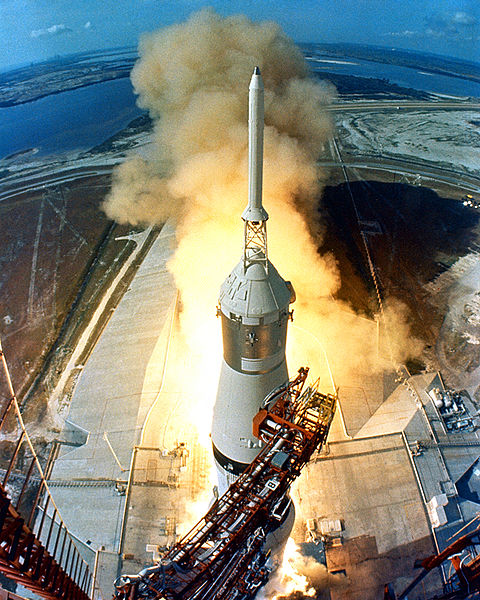
\includegraphics  [width=0.7\textwidth] {Images/Apollo_11_Launch2.jpg}
\end{figure}

\subsection{Deep Space One}
Deep Space One (DS-1), shown conceptually in \autoref{fig:DS-1}, was launched on 24 October 1998 with a mass of 374~kg \parencite{web_DS-1}. After launch, an electrostatic ion thruster took over propulsion on its one-way mission to the asteroid 9969~Braille and the comet 19P/Borrelly. This thruster generated 92~mN of thrust at a maximum input power of 2100~W. DS-1 had several similarities to the intended mission of \BW.

\begin{figure}[ht]
\caption{Deep Space One. Image used courtesy of NASA.}
\label{fig:DS-1}
\centering
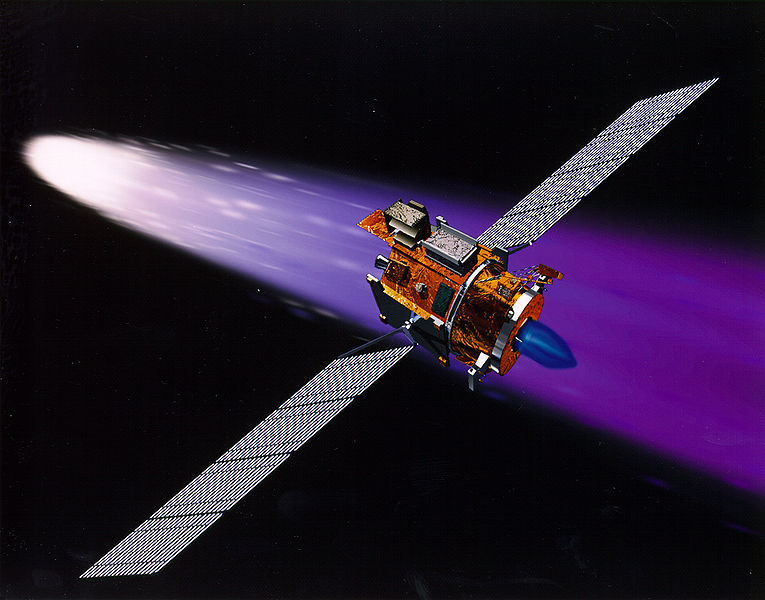
\includegraphics [width=0.7\textwidth] {Images/765px-Deep_Space_1_using_its_ion_engine.jpg}
\end{figure}
 
\textcite{Rayman1997} state that once or twice each week the spacecraft had to rotate away from its thrust vector in order to collect optical navigation pictures and communicate with the Deep Space Network (DSN) on Earth, which required shutting down the propulsion system. Key differences from \BW\ however, include the frequency and duration of these thrusting and coasting phases, and the nature of the trajectory. The interplanetary trajectory of DS-1 was dominated by a heliocentric orbit, with perturbations from the Earth, Mars and a number of asteroids. This means that the thrust vector was almost tangential to the orbital velocity around the Sun, and therefore the optimal orientation of solar panels (towards the Sun) was always perpendicular to the desired thrust vector (around the Sun). In contrast to this, \BW\ will occupy a cis-lunar orbit. This poses two difficulties: not only will the trajectory optimisation have to switch its reference frame from Earth-centric to lunar-centric in mid-flight, but optimal orientation of the solar panels relative to the direction of thrust is constantly changing. To overcome this the thrusting profile of \BW\ must shut down much more frequently than DS-1 did: hourly, rather than weekly, so that it can point its solar panels towards the Sun to recharge.

\subsection{Hayabusa}
Hayabusa (launched 9 May 2003), shown conceptually in \autoref{fig:Hayabusa}, was designed by the Japanese Aerospace Exploration Agency (JAXA) to perform a rendesvouz with asteroid 25143~Itokawa \parencite{web_Hayabusa}. It had a launch mass of 510~kg, including 130~kg of xenon gas used by the four microwave ECR (Electron Cyclotron Resonance) thrusters, providing 4$\times$8~mN = 32~mN thrust at maximum input power of 4$\times$350~W = 1400~W. Hayabusa had a similarly weak thrust to \BW, but was once again in a heliocentric orbit. Hayabusa successfully re-entered Earth's atmosphere and was recovered near Woomera, South Australia in June 2010, despite numerous failures including almost complete failure of all four ECR thrusters.

\begin{figure}[ht]
\caption{Japanese Hayabusa probe. Image used courtesy of J. Garry.}
\label{fig:Hayabusa}
\centering
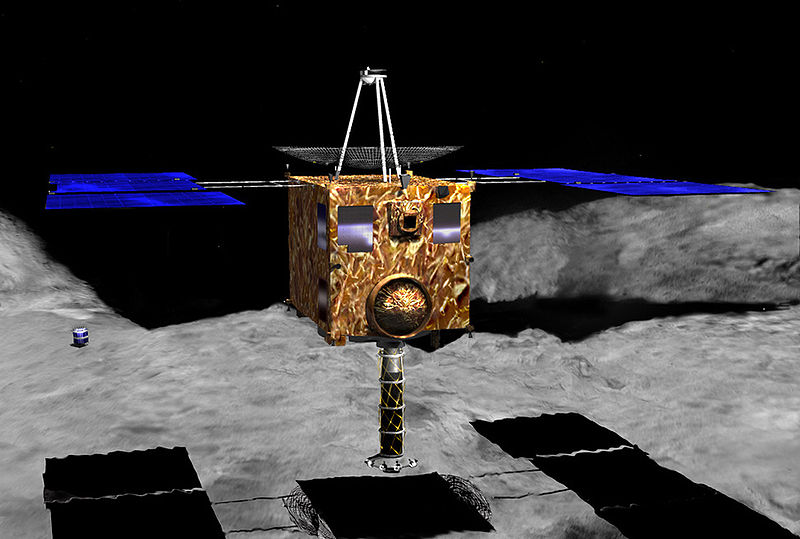
\includegraphics [width=0.7\textwidth] {Images/800px-Hayabusa_hover.jpg}
\end{figure}

\subsection{SMART-1}
Small Missions for Advanced Research in Technology One (SMART-1) (launched 27 September 2003) had a Hall effect plasma thruster providing 73~mN thrust at 1200~W power consumption \parencite{web_SMART-1}. The craft, shown conceptually in \autoref{fig:SMART-1}, was a comparable size to \BW, but twice as heavy: 367~kg including 80~kg of xenon propellant. On September 3, 2006 SMART-1 was deliberately crashed into the Moon's surface. This mission profile is closest to that intended for \BW, but had an order of magnitude higher thrust. \textcite{Estublier2007} provides a useful summary of SMART-1 performance data.

\begin{figure}[ht]
\caption{SMART-1. Image used courtesy of USGS.}
\label{fig:SMART-1}
\centering
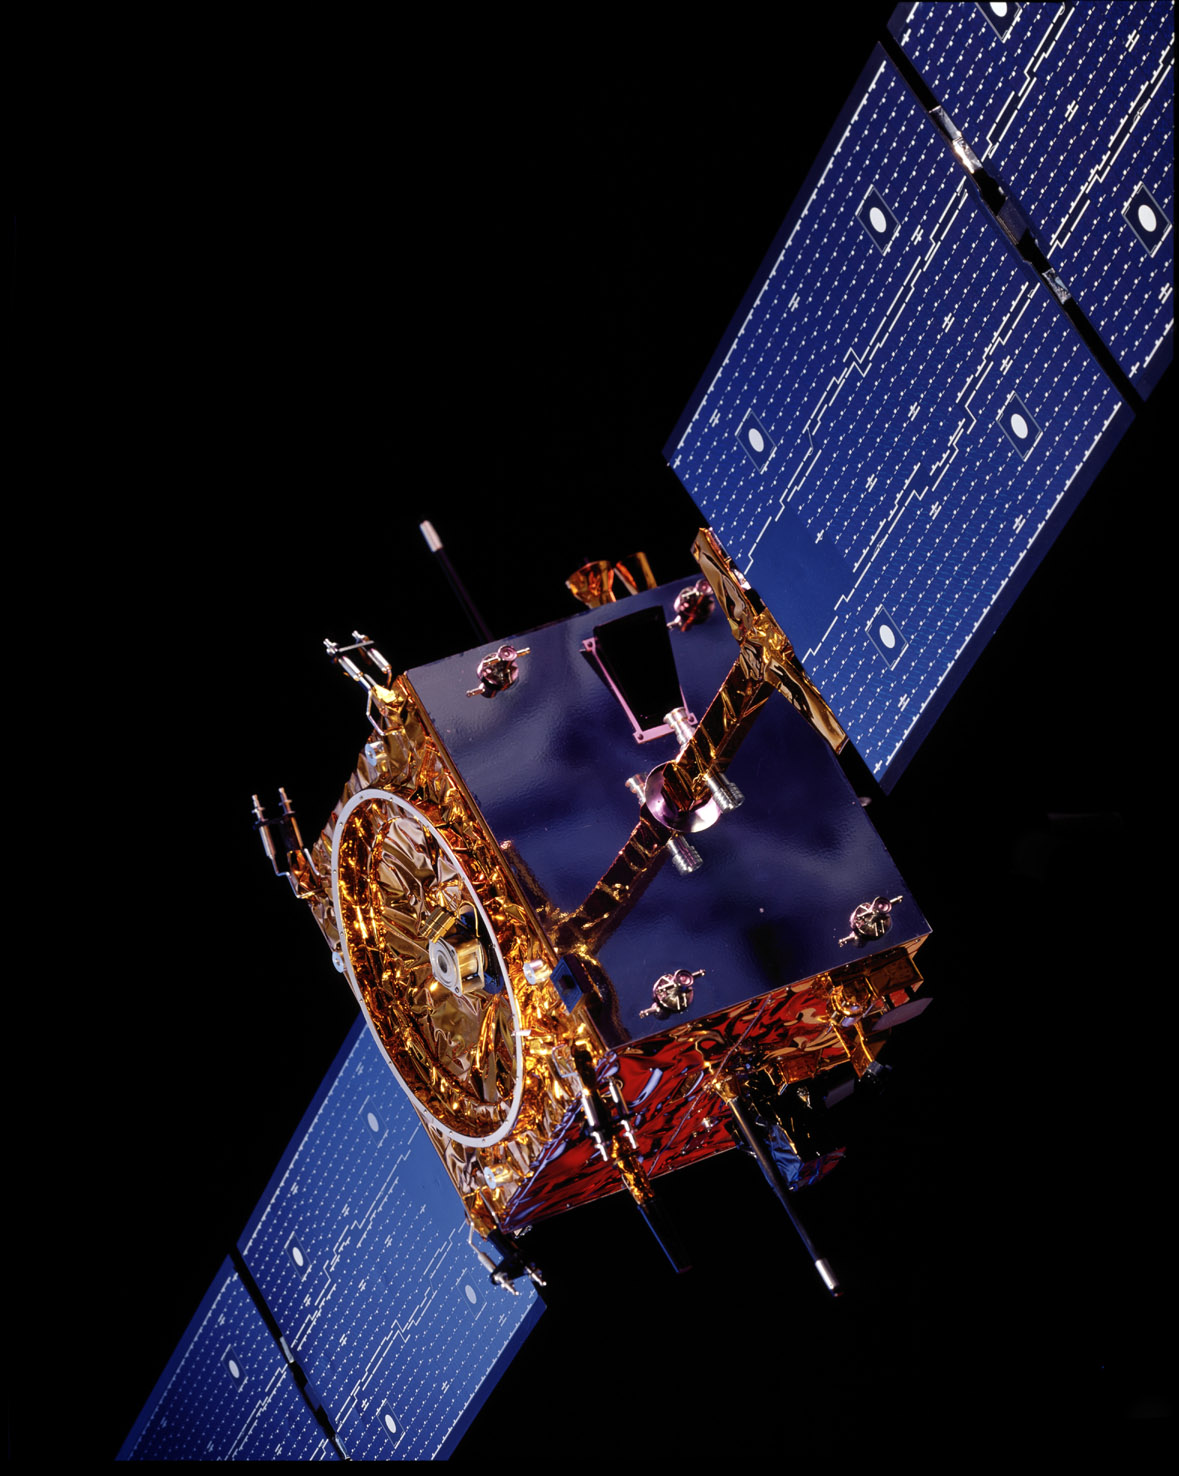
\includegraphics [angle=90,width=0.7\textwidth] {Images/SMART-1.jpg}
\end{figure}

\subsection{Dawn}
Dawn (launched 27 September 2007) is using the same thrusters developed for DS-1 to propel it towards the dwarf planet 1~Ceres by 2015 \parencite{web_Dawn}, following a successful rendezvous with the main-belt asteroid 4~Vesta in June 2011. Getting to Vesta it consumed 275~kg xenon, and will use another estimated 110~kg to get to Ceres, out of a total of 425~kg of on-board propellant. Dawn, shown conceptually in \autoref{fig:Dawn}, had a total launch mass of 1250~kg.

\begin{figure}[ht]
\caption{Dawn. Image used courtesy of NASA.}
\label{fig:Dawn}
\centering
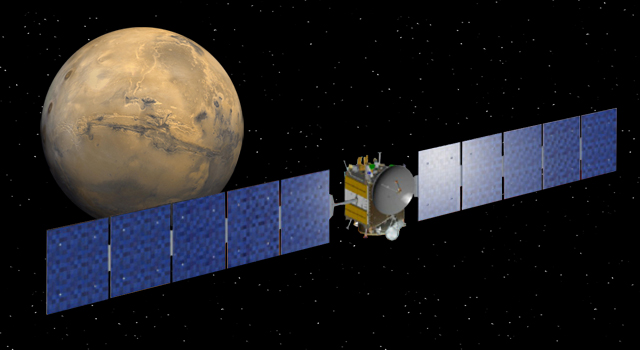
\includegraphics  [width=0.7\textwidth] {Images/mars-browse.jpg}
\end{figure}

\subsection{Planned missions}
Planned electrically propelled missions include SMART-2, also known as LISA Pathfinder \parencite{web_SMART-2}, and Space-Technology~7 (ST-7) to be launched by NASA. Common to all of these missions is thrust substantially higher than \BW\ will have available, and consequently \BW\ will have a less flexible escape trajectory.

\BW\ will be only the fifth electrically propelled spacecraft to leave Earth orbit, and the first mission with this type of electric propulsion.



% -------------------------------------------------------- Optimisation methods --------------------------------------------------------

\section{Optimisation methods} \label{sec:Optimisation-methods}

%\cite{Melbourne1962,Melbourne1965} Mars trajectories under solar gravity only
%Not much work on reduced three-body problem

%London and Stuhlinger - patched two-body segments
% \cite{Stuhlinger1964} cited by Herman1998

%Citing other peoples' graphs in Lit Review: .... Reproduced from \cite{}

Traditional high-thrust chemical rocket trajectories do not need optimisation for lunar missions, since the duration is sufficiently small that perturbing forces are negligible. In the resulting restricted three-body scenario (the Earth and Moon are static, with a spacecraft of negligible mass orbiting them) there are simple analytical solutions for the trajectory.

As outlined in \autoref{cha:Objectives} the task of optimising a low-thrust trajectory is somewhat more complex due to the long duration of forces acting on the spacecraft requiring lengthy integrations. For the reader unfamiliar with optimisation, an outline is provided in \autoref{cha:Optimisation}. Specific trajectory optimisation techniques available to accomplish this task are described in \autoref{sec:Process}. This section addresses how effective previous studies have found those methods to be, and how applicable they are to \BW.

Firstly there are a number of existing literature reviews compiled by other authors. \textcite{Betts1998} provides a generalised explanation of the different optimisation algorithms, without addressing any particular scenarios. 

\textcite{McKay2011} provide a survey of non-keplerian orbits, which they define as any orbit with forces additional to the primary point-mass gravitational force. Literature is included in this survey covering a broad spectrum of trajectory planning and optimisation from optimal control and sequential quadratic programming to genetic algorithms. Their study was focussed towards using low thrust propulsion to maintain a stable orbit in the presence of these secondary forces, and while \BW1 requires a transfer trajectory rather than a stable orbit their paper does conclude that there are some serious deficiencies with established research in the area: 

\begin{quotation}It is clear, however, that work still has to be done to transform the steadily growing body of literature on highly-non-Keplerian orbits from interesting theory into actual, practical missions.
\end{quotation}

The survey did not include analysis of any actual missions, but rather compared existing theoretical studies. For the purposes of this literature review, those studies and additional ones will be divided into indirect optimal control and gradient projection methods, direct nonlinear programming techniques, and other direct numerical techniques, as defined in \autoref{sec:Process}.






% Optimal control
\subsection{Optimal control and gradient projection methods} \label{sub:Optimal-control-lit}

As mentioned, chemical rocket trajectories do not generally need optimisation for lunar missions. Interplanetary missions are a different matter entirely, as gravitational assists can lead to a very complex solution space. The traditional approach is by patching simplified two-body segments together. Consequently, this technique was widely used to apply optimal control theory to low-thrust trajectory optimisation, such as that performed by \textcite{Stuhlinger1964}. However, many technological hurdles emerged restricting the uptake of electrical propulsion systems on spacecraft, so interest in the topic waned.

Most of these hurdles had been overcome by the early 1990s. \textcite{Golan1994} resumed trajectory planning by optimal control for low-thrust spacecraft, starting from an analytical solution developed by \textcite{Breakwell1966}. \citeauthor{Golan1994} expanded on the previous work by patching two optimally-controlled spirals together in an Earth-Moon fixed frame, albeit assuming a specific thrust of $9.81\times10^{-3}\text{ ms}^{-2}$, over 200 times more thrust per kilogram than \BW\ will have. While their trajectory analysis does allow for a variable thrust engine, it does not consider practical issues such as coasting phases to recharge the batteries, or transits through the Earth's shadow. The larger thrust allows a much shorter transfer time than anticipated for \BW, so weaker perturbations such as the Earth's oblateness and the gravitational pull of the Sun and Jupiter were neglected.

\textcite{Guelman1995} performed a similar optimal control based trajectory analysis within a three-body plane. An interesting difference to \citeauthor{Golan1994}'s approach is that \citeauthor{Guelman1995} centred his coordinate system at the Earth-Moon barycentre. This smoothes the equations of motion in the region where the Earth and Moon have comparable influence on the spacecraft; however, since a lunar transfer generally spends very little time in this region, it is usually preferable to model with the conceptually easier Earth- and lunar-centred frames.
 
\citeauthor{Guelman1995} still uses a very simplified gravitational model, with a continuously thrusting spacecraft. Variable thrust is allowed for by minimising the total thrust required to achieve a lunar orbit/impact given a constant thrust duration. While this approach achieved lower magnitude thrust profiles than \citeauthor{Golan1994} (for 1000 hours of thrust \citeauthor{Guelman1995} found a maximum of $4.3\times10^{-3}\text{ ms}^{-2}$ was required), it is inappropriate in the current scenario since the mission is constrained by impulse (total thrust delivered over the flight) rather than thrust magnitude. Furthermore, calculating the gravitational field within a barycentric frame becomes increasingly complex with the number of bodies in the gravitational model, making it unsuitable for very low thrust missions which must allow for the weaker perturbations mentioned above.

\textcite{Guelman2000} improved on their gravitational model by time averaging the effects of gravity and thrust, ignoring the short term cyclical changes and focussing instead on the slower changes of orbital elements and thrust profile. This scenario was then solved via Pontryagin's Maximum Principle using their own SQP procedure. However, even with this simplification he ran into severe computational problems, requiring \enquote{about 100,000 evaluations of trigonometric integrands per integration node. Thus even a modest number of nodes, say 100 per trajectory, requires significant time expenditure}. 

In contrast, \textcite{Pierson1994} simplified the optimal control problem by breaking it into three two-dimensional stages. These three stages consisted of a constant thrust Earth-escape, a cis-lunar coast, and a constant thrust lunar capture. This method was extended to a full three-dimensional problem by \textcite{Kluever1995,Kluever1996,Kluever1997}. However, all of these papers assume a continuous thrust profile which is incompatible with both \BW's thrust constraints, and the inherent restrictions placed on thrusting by passing through the Earth's shadow. Furthermore, the optimisation method developed in these papers is adapted from \textcite{Edelbaum1964}, using curve fitting to develop an approximate solution with much less computational effort than the analytical methods utilised previously. Sequential quadratic programming is then used to solve the curve-fitted problem.

The starting conditions of 100,000~kg with 2942~N of electric propulsion pose a confusingly ambitious scenario, given the magnitude of thrust available from current electric propulsion systems and the expectation of sending a mass similar to that of the International Space Station to the Moon. Worthy of note, however, is their utilisation of backwards propagation to assist with achieving lunar capture. To ensure strong capture, their optimisation minimised orbital energy with respect to the Moon over a fixed time. Within their two-dimensional model, they investigated the difference between targeting posigrade and retrograde about the Moon, and found a slight advantage in the posigrade orbit (final LLO mass of 93,092~kg compared with 93,032~kg for retrograde). Both scenarios improved on their respective initial guesses by less than 10~kg (about 0.1\%) suggesting that either the optimisation method employed was not particularly effective, or the problem was particularly smooth and very little improvement could be made. 

The papers of \textcite{Kluever1995, Kluever1996} adapt the solution technique into a hybrid approach. First an experimental procedure is presented to find an initial guess. The trajectory under full thrust is simulated, and the phase time increased until the spacecraft gets near the lunar sphere of influence (SOI, defined in \autoref{sec:SOI}). The simulation is extended with no thrust to observe the lunar fly-by, and the initial angle is adjusted (in a 2D moon-fixed frame) until the coasting trajectory enters the SOI with a negative radial velocity relative to the Moon. The process is then repeated in reverse for the lunar descent, and the problem then becomes making the two trajectories meet in the middle. This two dimensional solution technique assumes that the initial orbit of the spacecraft about the Earth is coplanar with the Moon's orbit. Many other simplifications are made, such as neglecting external forces. These simplifications were required so that the inverse costate equations could be found allowing Pontryagin's principle to be exploited, giving a very accurate initial guess for the thrust profiles in ascent and descent phases. SQP was then used to blend the phases together. All of these papers assume the (very large) spacecraft can deliver constant thrust and constant mass flow. They do not address initial launch conditions such as inclination, not to mention the feasibility of launching such a mass in the first place.

\textcite{Kluever1997} extended the work to three dimensions, and even targeted a polar lunar orbit. The transfer still starts from very high earth orbit, and still implements a thrust-to-weight ratio of $1.3\times10^{-4}$~ms$^{-2}$, much higher than \BW\ will have available. Pontryagin necessary conditions were used to parameterise the intial guess control profile, but the problem was then solved entirely using direct optimisation. The initial guess is based on the 2D optimisations for a GEO-HLO transfer, with the plane change occuring during the HLO-LLO descent phase. During optimisation the plane change slowly adjusted from the HLO-LLO phase until it is almost entirely included in GEO-HLO phase, demonstrating the efficiency of trajectory targeting maneouvres in cis-lunar space.

% Conclusion - shortcomings of indirect methods leading in to direct? No, not making that distinction here. 




\subsection{Nonlinear programming and sequential quadratic programming methods} \label{sub:NLP-lit}

\textcite{Enright1992} parameterised the state and control variables with a piecewise polynomial, thus establishing a collocation method. Extensive work is then dedicated to demonstrating that the resulting nonlinear problems approximate the optimal control problem, and that the Lagrange multipliers are equivalent to the Pontryagin adjoint variables. A number of scenarios including an Earth-Moon transfer are then presented to verify their Hermite-Simpson direct transcription technique and Runge-Kutta parallel shooting technique. 

\citeauthor{Enright1992} conclude by identifying some shortcomings of their study: \enquote{it is desirable to solve lunar transfer problems for lower thrust levels, lower initial and final orbit radii, and for the noncoplanar case. The main obstacle is the size of the nonlinear programming problem that results. (Other enhancements, such as lunar eccentricity and a better Earth gravity potential, do not affect the problem size.)}
They go on to outline how solving these larger problems may be accomplished. \enquote{First, the previous problem was solved using uniform mesh point distribution within a phase (and also the same number of mesh points for each phase). The data suggest that this is extremely inefficient, and an intelligent redistribution should be performed. Second, the NLP algorithm NPSOL is not designed to handle large sparse problems efficiently. The authors have had some success with the MINOS package that is designed for large-scale systems, and we recommend it for problems with more than 400 variables. Finally, alternate coordinate systems could be employed to possibly increase the smoothness of the solution, reducing the number of mesh points required. A variation-of-parameters approach or other strategies might be attempted.}
%lunar eccentricity and better geopotential do not affect problem size (just time to solve; longer computation each step, but doesn't increase the number of steps).

\textcite{Herman1998} use what they describe as a \enquote{very low} thrust magnitude of $10^{-4}$~g. They identify lower thrust increases the size of the problem, and consequently the difficulty. However, their entire transfer takes only 32~days, with 9~Earth orbits and 7~lunar orbits. Nonetheless,the problem is solved using collocation to transcribe the optimal control problem into non-linear subproblems. It implements constant thrust and then optimises for time, which has the same effect as optimising for fuel use. The non-linear problems are solved using a proprietary McDonnell-Douglas optimisation algorithm called NZOPT. Despite the simpler scenario, this study does establish collocation and nonlinear programming as a promising approach to solving the low-thrust trajectory optimisation problem.

\textcite{Betts1993} investigated computationally efficient numerical techniques to determine near-optimal trajectories, by exploiting sparsity within the Jacobian and Hessian matrices. In particular, they utilised direct transcription and collocation to approximate the optimisation problem, which was then solved numerically using sparse nonlinear programming.
 
\textcite{Betts1994} introduced a package called Sparse Optimal Control Software (SOCS), and concluded that it is a very computationally efficient method for numerically optimising low-thrust trajectories that include non-linearities caused by perturbing forces. This appears to be a very promising approach, but \textcite{Betts2000} acknowledges that none of these papers included tesseral harmonics of the Earth's gravitational field, third-body gravitational perturbations from the Sun, Moon, or Jupiter, variable thruster duty cycles, the Earth's shadow limits, or atmospheric drag at low altitudes. These papers all used an orbit-to-orbit transfer, with a spacecraft thrusting
 at $1.25\times10^{-4}\text{ ms}^{-2}$ as a test case (this is still an order of magnitude greater thrust than \BW).

The direct transcription approach of \textcite{Betts1993} was extended by \textcite{Erb_thesis} and then \textcite{Betts2003}, by optimising a lunar transfer from GTO employing solar electric propulsion; a mission profile very similar to that of SMART-1. These papers verified that the direct transcription method with sparse non-linear programming is a suitable approach for low-thrust lunar missions, but once again assumed constant thrust throughout the transfer, ignoring Earth shadowing, as well as neglecting tesseral Earth harmonics. While this method may be useful for optimising \BW, as a numerical approach it is not guaranteed to find the optimal path. The performance is also heavily reliant on the initial guess, as highlighted by \textcite{Betts2003}: 

\begin{quotation}The design of an initial guess for a trajectory with a vast number of revolutions, significant inclination changes, capturing and orbital corrections is a challenging task on its own.\end{quotation}

\textcite{Letterio_thesis} described the optimisation of a low thrust transfer using an identical thrust regime to \BW\ (in fact, \citeauthor{Letterio_thesis}'s study was completed as part of the same project with Universit\"{a}t Stuttgart). However, his study only covers the ascent phase, from geosynchronous transfer orbit (GTO) to the outer limits of the van Allen belts, using the higher thrust arcjet. The emphasis was on increasing the radius of the orbit as quickly as possible to escape the van Allen belts. Furthermore, at these relatively low altitudes the gravitational perturbations due to the Moon's gravity are fairly uniform. This limits the extent to which they can be exploited to optimise the trajectory of the spacecraft.

An interesting series of articles in \emph{Acta Astronautica} describe a competition devised by ESA to develop a benchmark test for low thrust optimisation. As the winners of the inaugural competition, held in 2007, \textcite{Petropoulos2007} summarised their findings: 

\begin{quotation}...it seems that a rough global search, based on simple numerical schemes coupled with mission design intuitions, is a necessary precursor activity to the local optimisation, and one which is a rich area for research.\end{quotation}

The 2007 competition was dominated by gravity assists to maximise a spacecraft's velocity, and as such is most relevant to inter-planetary low-thrust trajectories. Several entries attempted to optimise direct transfers from Earth to the target orbit, a scenario with similarities to the planned lunar transfer of \BW. In particular, \textcite{Dachwald2007} developed a program that combines evolutionary algorithms and neural networks to search for an optimal thrust profile. Despite the apparent failure of this method in the competition, their diagnosis of the resulting trajectory demonstrates key aspects of exploiting gravitational perturbations. Due to the short timescale of the competition this research was not continued.






\subsection{Other methods} \label{sub:Other-lit}

There are of course many alternatives to gradient based methods of optimisation. Techniques such as genetic algorithms and simulated annealing have attracted an increasing amount of interest in recent decades, as outlined by \textcite{Ren2007}. The primary advantage of these methods is that they provide a better global search before descending into a basin of convergence. Unfortunately there is still no way to be certain that the basin selected will have a better optimum than others, however an implicit assumption that the gradient is generally fairly uniform across the search area (that is, the problem is not very stiff) suggests that the basin with a better objective function at the top will have a better objective function at the bottom also. The assumption of a non-stiff search area also implies that the optimal solution will be located at the bottom of the widest basin of convergence, which is additionally the most likely to be found by the search algorithm.

An interesting methodological approach to optimisation is presented by \textcite{Jackson2008}. Rather than developing an analytic equation to optimise, or a numerical algorithm to iteratively determine a search direction, a coarse mesh of possible trajectories is plotted based on a few controlled parameters. The largest basin of convergence is then selected based on the assumption that it will be the most robust - even if the global optimum is found using another technique, the spacecraft will never be able to follow that trajectory \emph{exactly}. If the basin of convergence is too narrow, any number of unexpected events could easily push the spacecraft onto a severely sub-optimal trajectory, potentially resulting in the spacecraft not completing its mission. Iteratively calculating trajectories over a mesh of possible launch parameters determines a near-optimal trajectory, within a very broad basin of convergence. While the test case used by \textcite{Jackson2008} involved continual thrust from Earth orbit to the Sun-Earth libration point L1, the methodological nature of this approach allows easy implementation of discontinuous thrust profiles for \BW.%This will allow experimentation with exploiting lunar gravitational assists, as well as multiple non-linearities ignored or neglected in previous studies.

\textcite{Lee2005} performed a number of interplanetary trajectory optimisations using the more commonplace direct methods of genetic algorithms and simulated annealing. He points out that evolutionary algorithms often need distributed computing environments due to the number of computations involved. Computing power is becoming cheaper, but the parameterised problems are becoming larger. 

Reviewed literature such as \textcite{Dachwald2005} and \textcite{Jackson2008} has shown an increasing trend using these direct methods to perform a global search identifying the most promising basins of convergence. However, depending on the implementation direct methods often have difficulty determining the local optimum within the basin. 
Consequently there is a large and promising body of work utilising direct methods for global search, followed by indirect gradient methods to find the local optima within those basins \parencite{Stryck1992, Kluever1995, Vasile2009, Yam2011}.

%\cite{Yam2011} attempts global search using basin hopping and simulated annealing, each hybridized with a local search algorithm. Has to approximate the low thrust maneouvre as a series of impulsive maneouvers. cartesian state. theoretical nuclear electric mission to Jupiter, 2.26~N, 6000~s, 20000~kg with gravitational swing-bys. another one to Mercury, 1300~kg, 0.34~N and 3200~s.

\subsection{Summary of optimisation methods}

There is a vast amount of literature on low thrust trajectory optimisation. Early efforts focussed on indirect optimal control theory, which was soon discretised and solved with numerical gradient techniques. Algorithms have been improving to allow more complex higher order problems to be solved using these techniques. Meanwhile, much work has been done recently developing direct optimisation techniques. These allow more flexibility in modelling, as required by the complexity of orbital dynamics, and can tolerate stiffer problems with undulating solution spaces. 

Unfortunately the genetic algorithm implemented in GESOP is still quite experimental. Consequently the project proceeding using the sparse optimal control software more suitable for higher order problems. This required determination of an intial guess for every optimisation, requiring thorough knowledge of orbital dynamics and the forces acting on the spacecraft throughout the transfer, and the mechanics of lunar capture.



% Summary
\section{Summary of gaps in existing knowledge}

There is a variety of literature on trajectory optimisation for low-thrust space vehicles, although surprisingly few reports have been written on the trajectory optimisation of missions launched over the last decade. Consequently, the majority of literature is highly theoretical, and in most cases heavily simplified. 

Early research in low-thrust trajectory optimisation consisted of analytical optimisation on two dimensional, two-body and restricted three-body scenarios. As more complex perturbing forces were included, the non-linearity of the functions to be optimised increased dramatically. More recent papers have resorted to numerical optimisation techniques. These numerical techniques are very computationally intensive, and are not guaranteed to find an optimal solution.

Even when these studies have included perturbing forces, they have been viewed as an unfortunate side-effect of space travel. Certainly, they do complicate the mathematics of spacecraft trajectory planning. As the spacecraft thrust becomes smaller and the transfer duration increases, the influence of external perturbing forces becomes larger. With an electric propulsion system as weak as that onboard \BW, the perturbing force of the Moon's gravity can dominate the thrust. Consequently, it seems appropriate to search for a computationally efficient method to exploit these perturbing forces to increase the spacecraft's orbital velocity and radius.